\chapter{系统测试与分析}

\section{系统测试环境}

我们的系统基于 Microsoft 开源的 Deepspeed 框架 \ucite{deepspeed} 进行开发,主要使用 Python 语言。我们使用了一个 8 层的 Transformer-xl 模型 \ucite{dai2019transformer},并在其基础上拓展成为 MoE 架构。
在数据集的选择上,我们主要使用了 enwik8 数据集 \ucite{enwik8} 进行测试。

我们使用了私有集群进行测试,其中包括两种不同的 GPU 集群配置,用于验证基于网络拓扑的自动负载均衡策略设计。我们主要使用了 2 节点 8 卡的 Nvidia Titan XP GPU 集群以及 4 节点 8 卡的 Nvidia Titan XP GPU 集群。集群节点之间的网络通信通过Ethernet,其带宽约为10Gb/s。

\section{系统性能指标}

我们主要关注两个性能指标进行测试。第一个指标是模型的收敛速度,即 loss 收敛速度。第二个指标是每个 step 的完成时间,即模型训练过程中每个batch所需要的forward + backward + gradient synchronization所需要的总时间。我们将对这两个指标进行详细的测试评估,并根据测试结果进行优化和调整。

\section{实验结果}

\subsection{动态路由的数据分派策略实验结果}

我们进行了动态路由的数据分派策略实验,并将我们的设计与传统的Top-1和Top-2 Gating策略进行了对比。实验的对象是Transformer-XL模型,我们关注了每轮训练中损失的变化情况,并将其可视化为图表。

\begin{figure}[h!]
    \vskip 2ex
    \centering
    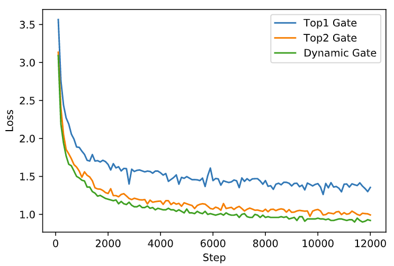
\includegraphics[width=0.7\linewidth]{figures/fig9.png}
    \caption{训练Loss变化图}
    \label{fig-loss}
    \end{figure}

    对比传统的Top-1和Top-2 Gating策略,我们的设计采用了动态路由的数据分派策略。通过实验结果的对比分析,我们发现我们的设计在损失的降低速度和最终的收敛效果上表现出了显著的优势。图\ref{fig-loss}清晰地展示了每轮训练中损失的变化趋势,我们的设计在较早的轮次就取得了更快的收敛速度,并且在后续的训练过程中持续保持较低的损失值。

这些实验结果表明,我们的动态路由数据分派策略在Transformer-XL模型上的有效性和优越性。相比传统的Top-1和Top-2 Gating策略,我们的设计能够更好地调度和分配数据,使得模型能够更快地收敛并获得更好的训练效果。这为提升模型性能和训练效率提供了有力的实证支持。

综上所述,我们的动态路由数据分派策略在Transformer-XL模型上的实验结果显示出了明显的优势,为改进模型训练和优化数据分派提供了一种有效的方法。这些发现对于深度学习研究和实践具有重要意义,并为未来的工作和改进方向提供了有益的启示。

\subsection{基于网络拓扑的自动负载均衡实验结果}

\subsubsection{端到端训练性能分析}
我们对基于网络拓扑的自动负载均衡设计在GPU集群上进行了测试,我们使用了2个节点,每个节点配备了8个Nvidia TitanX GPU。网络带宽为10Gbps,训练框架采用了Deepspeed,MoE模型为Transformer-xl MoE,数据集为enwik8,模型参数量为45M。

根据我们的实验数据\ref{fig-breakdown},我们的设计在前向传播阶段获得了约4.09倍的加速比。这表明我们基于网络拓扑的自动负载均衡设计在模型的前向计算过程中取得了显著的性能提升。通过有效地分配计算任务和利用GPU集群的并行能力,我们能够加快前向传播的速度,从而加速整体训练过程。

\begin{figure}[h!]
    \vskip 2ex
    \centering
    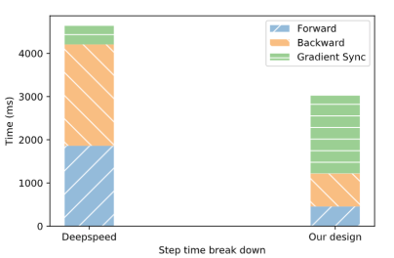
\includegraphics[width=0.7\linewidth]{figures/fig10.png}
    \caption{参数量为45M时,每个step时间步分解}
    \label{fig-breakdown}
    \end{figure}

在后向传播阶段,我们的设计获得了约3.08倍的加速比。这进一步证明了我们的自动负载均衡设计在处理梯度计算和参数更新时的优越性。通过合理地分配计算任务和优化通信流程,我们能够有效地利用GPU集群的计算资源,提高后向传播的效率。

然而,在梯度同步阶段,由于更负载的并行策略和更复杂的通信流程,我们的设计可能会遇到一定程度的性能下降。这是因为梯度同步过程中的通信开销增加,可能导致整体训练速度的一定减缓。

综合而言,基于我们的实验结果,我们的基于网络拓扑的自动负载均衡设计在前向传播和后向传播阶段分别获得了约4.09倍和3.08倍的加速比。虽然在梯度同步阶段可能存在一定的性能下降,但最终整体端到端的训练速度仍然提升了约1.24倍。这证明了我们设计的有效性和优越性,能够加速训练过程并提高模型训练的效率。在未来的工作中,我们将继续优化和改进设计,以进一步提高整体训练速度并减少梯度同步阶段的性能下降。

\begin{table}[]
    \centering
    \label{table-45M}
    \caption{在参数量为45M的Trasnformer-xl MoE模型训练中,我们的设计与baseline(Deepspeed)的Step Time的拆分}
    \begin{tabular}{|
    >{\columncolor[HTML]{FFFFFF}}l |
    >{\columncolor[HTML]{FFFFFF}}l |
    >{\columncolor[HTML]{FFFFFF}}l |
    >{\columncolor[HTML]{FFFFFF}}l |}
    \hline
    {\color[HTML]{333333} Stages}             & {\color[HTML]{333333} Baseline} & {\color[HTML]{333333} Our design} & {\color[HTML]{333333} \textbf{Acc}}   \\ \hline
    {\color[HTML]{333333} Fwd\_MoE (ms)} & {\color[HTML]{333333} 1860} & {\color[HTML]{333333} 455}  & {\color[HTML]{333333} \textbf{4.09x}} \\ \hline
    {\color[HTML]{333333} Bwd\_Moe (ms)} & {\color[HTML]{333333} 2347} & {\color[HTML]{333333} 761}  & {\color[HTML]{333333} \textbf{3.08x}} \\ \hline
    {\color[HTML]{333333} Gradient Sync (ms)} & {\color[HTML]{333333} 430}      & {\color[HTML]{333333} 1805}       & {\color[HTML]{333333} \textbf{0.24x}} \\ \hline
    {\color[HTML]{333333} Overall (ms)}  & {\color[HTML]{333333} 5200} & {\color[HTML]{333333} 3576} & {\color[HTML]{333333} \textbf{1.45x}} \\ \hline
    \end{tabular}
    \end{table}

\subsubsection{自动负载均衡策略深入分析}

\begin{sidewaystable}
    \centering
    \begin{adjustbox}{max width=0.8\textwidth}
        \begin{tabular}{@{}|
            >{\columncolor[HTML]{FFFFFF}}l 
            >{\columncolor[HTML]{FFFFFF}}l 
            >{\columncolor[HTML]{FFFFFF}}l 
            >{\columncolor[HTML]{FFFFFF}}l |
            >{\columncolor[HTML]{FFFFFF}}l 
            >{\columncolor[HTML]{FFFFFF}}l 
            >{\columncolor[HTML]{FFFFFF}}l 
            >{\columncolor[HTML]{FFFFFF}}l 
            >{\columncolor[HTML]{FFFFFF}}l 
            >{\columncolor[HTML]{FFFFFF}}l 
            >{\columncolor[HTML]{FFFFFF}}l 
            >{\columncolor[HTML]{FFFFFF}}l 
            >{\columncolor[HTML]{FFFFFF}}l |@{}}
            \toprule
            \multicolumn{2}{|l|}{\cellcolor[HTML]{FFFFFF}{\color[HTML]{333333} 8 GPUs 2 Nodes}} &
              \multicolumn{2}{l|}{\cellcolor[HTML]{FFFFFF}model: transformer-xl} &
              \multicolumn{2}{l|}{\cellcolor[HTML]{FFFFFF}layer:8} &
              \multicolumn{2}{l|}{\cellcolor[HTML]{FFFFFF}batch\_size: 24} &
              \multicolumn{5}{l|}{\cellcolor[HTML]{FFFFFF}} \\ \midrule
            \multicolumn{1}{|l|}{\cellcolor[HTML]{FFFFFF}} &
              \multicolumn{3}{l|}{\cellcolor[HTML]{FFFFFF}Fwd\_MoE(ms)} &
              \multicolumn{3}{l|}{\cellcolor[HTML]{FFFFFF}Bwd\_inner(ms)} &
              \multicolumn{3}{l|}{\cellcolor[HTML]{FFFFFF}Bwd\_Allreduce (ms)} &
              \multicolumn{3}{l|}{\cellcolor[HTML]{FFFFFF}Overall (ms)} \\ \cmidrule(l){2-13} 
            \multicolumn{1}{|l|}{\multirow{-2}{*}{\cellcolor[HTML]{FFFFFF}\#Params}} &
              \multicolumn{1}{l|}{\cellcolor[HTML]{FFFFFF}Baseline} &
              \multicolumn{1}{l|}{\cellcolor[HTML]{FFFFFF}Our   design} &
              Acc &
              \multicolumn{1}{l|}{\cellcolor[HTML]{FFFFFF}Baseline} &
              \multicolumn{1}{l|}{\cellcolor[HTML]{FFFFFF}Our   design} &
              \multicolumn{1}{l|}{\cellcolor[HTML]{FFFFFF}Acc} &
              \multicolumn{1}{l|}{\cellcolor[HTML]{FFFFFF}Baseline} &
              \multicolumn{1}{l|}{\cellcolor[HTML]{FFFFFF}Our   design} &
              \multicolumn{1}{l|}{\cellcolor[HTML]{FFFFFF}Acc} &
              \multicolumn{1}{l|}{\cellcolor[HTML]{FFFFFF}Baseline} &
              \multicolumn{1}{l|}{\cellcolor[HTML]{FFFFFF}Our   design} &
              Acc \\ \midrule
            \multicolumn{1}{|l|}{\cellcolor[HTML]{FFFFFF}45M} &
              \multicolumn{1}{l|}{\cellcolor[HTML]{FFFFFF}1860} &
              \multicolumn{1}{l|}{\cellcolor[HTML]{FFFFFF}455} &
              \textbf{4.09x} &
              \multicolumn{1}{l|}{\cellcolor[HTML]{FFFFFF}2347} &
              \multicolumn{1}{l|}{\cellcolor[HTML]{FFFFFF}761} &
              \multicolumn{1}{l|}{\cellcolor[HTML]{FFFFFF}\textbf{3.08x}} &
              \multicolumn{1}{l|}{\cellcolor[HTML]{FFFFFF}430} &
              \multicolumn{1}{l|}{\cellcolor[HTML]{FFFFFF}1805} &
              \multicolumn{1}{l|}{\cellcolor[HTML]{FFFFFF}\textbf{0.24x}} &
              \multicolumn{1}{l|}{\cellcolor[HTML]{FFFFFF}5200} &
              \multicolumn{1}{l|}{\cellcolor[HTML]{FFFFFF}3576} &
              \textbf{1.45x} \\ \midrule
            \multicolumn{1}{|l|}{\cellcolor[HTML]{FFFFFF}94M} &
              \multicolumn{1}{l|}{\cellcolor[HTML]{FFFFFF}1929} &
              \multicolumn{1}{l|}{\cellcolor[HTML]{FFFFFF}463} &
              \textbf{4.17x} &
              \multicolumn{1}{l|}{\cellcolor[HTML]{FFFFFF}2386} &
              \multicolumn{1}{l|}{\cellcolor[HTML]{FFFFFF}815} &
              \multicolumn{1}{l|}{\cellcolor[HTML]{FFFFFF}\textbf{2.93x}} &
              \multicolumn{1}{l|}{\cellcolor[HTML]{FFFFFF}430} &
              \multicolumn{1}{l|}{\cellcolor[HTML]{FFFFFF}5350} &
              \multicolumn{1}{l|}{\cellcolor[HTML]{FFFFFF}\textbf{0.08x}} &
              \multicolumn{1}{l|}{\cellcolor[HTML]{FFFFFF}5161} &
              \multicolumn{1}{l|}{\cellcolor[HTML]{FFFFFF}7005} &
              \textbf{0.74x} \\ \bottomrule
        \end{tabular}
    \end{adjustbox}
    \label{table-dive-deep-param}
    \caption{更改模型参数,分析系统训练性能}
    
% \end{sidewaystable}

\bigskip
% \begin{sidewaystable}
    \centering
    \begin{adjustbox}{max width=0.8\textwidth}
        \begin{tabular}{@{}|
            >{\columncolor[HTML]{FFFFFF}}c 
            >{\columncolor[HTML]{FFFFFF}}c 
            >{\columncolor[HTML]{FFFFFF}}c 
            >{\columncolor[HTML]{FFFFFF}}c |
            >{\columncolor[HTML]{FFFFFF}}c 
            >{\columncolor[HTML]{FFFFFF}}c 
            >{\columncolor[HTML]{FFFFFF}}c 
            >{\columncolor[HTML]{FFFFFF}}c 
            >{\columncolor[HTML]{FFFFFF}}c 
            >{\columncolor[HTML]{FFFFFF}}c 
            >{\columncolor[HTML]{FFFFFF}}c 
            >{\columncolor[HTML]{FFFFFF}}c 
            >{\columncolor[HTML]{FFFFFF}}c |@{}}
            \toprule
            \multicolumn{2}{|c|}{\cellcolor[HTML]{FFFFFF}{\color[HTML]{333333} \textbf{8 GPUs 2 Nodes}}} &
              \multicolumn{2}{c|}{\cellcolor[HTML]{FFFFFF}\textbf{model: transformer-xl}} &
              \multicolumn{2}{c|}{\cellcolor[HTML]{FFFFFF}\textbf{layer:8}} &
              \multicolumn{2}{c|}{\cellcolor[HTML]{FFFFFF}\textbf{batch\_size: 40}} &
              \multicolumn{5}{l|}{\cellcolor[HTML]{FFFFFF}} \\ \midrule
            \multicolumn{1}{|c|}{\cellcolor[HTML]{FFFFFF}} &
              \multicolumn{3}{c|}{\cellcolor[HTML]{FFFFFF}Fwd\_MoE (ms)} &
              \multicolumn{3}{c|}{\cellcolor[HTML]{FFFFFF}Bwd\_inner (ms)} &
              \multicolumn{3}{c|}{\cellcolor[HTML]{FFFFFF}Bwd\_Allreduce (ms)} &
              \multicolumn{3}{c|}{\cellcolor[HTML]{FFFFFF}Overall (ms)} \\ \cmidrule(l){2-13} 
            \multicolumn{1}{|c|}{\multirow{-2}{*}{\cellcolor[HTML]{FFFFFF}\#Params}} &
              \multicolumn{1}{c|}{\cellcolor[HTML]{FFFFFF}Baseline} &
              \multicolumn{1}{c|}{\cellcolor[HTML]{FFFFFF}Our design} &
              Acc &
              \multicolumn{1}{c|}{\cellcolor[HTML]{FFFFFF}Baseline} &
              \multicolumn{1}{c|}{\cellcolor[HTML]{FFFFFF}Our design} &
              \multicolumn{1}{c|}{\cellcolor[HTML]{FFFFFF}Acc} &
              \multicolumn{1}{c|}{\cellcolor[HTML]{FFFFFF}Baseline} &
              \multicolumn{1}{c|}{\cellcolor[HTML]{FFFFFF}Our design} &
              \multicolumn{1}{c|}{\cellcolor[HTML]{FFFFFF}Acc} &
              \multicolumn{1}{c|}{\cellcolor[HTML]{FFFFFF}Baseline} &
              \multicolumn{1}{c|}{\cellcolor[HTML]{FFFFFF}Our design} &
              Acc \\ \midrule
            \multicolumn{1}{|c|}{\cellcolor[HTML]{FFFFFF}45M} &
              \multicolumn{1}{c|}{\cellcolor[HTML]{FFFFFF}3233} &
              \multicolumn{1}{c|}{\cellcolor[HTML]{FFFFFF}527} &
              \textbf{6.13x} &
              \multicolumn{1}{c|}{\cellcolor[HTML]{FFFFFF}4171} &
              \multicolumn{1}{c|}{\cellcolor[HTML]{FFFFFF}1146} &
              \multicolumn{1}{c|}{\cellcolor[HTML]{FFFFFF}\textbf{3.64x}} &
              \multicolumn{1}{c|}{\cellcolor[HTML]{FFFFFF}430} &
              \multicolumn{1}{c|}{\cellcolor[HTML]{FFFFFF}1813} &
              \multicolumn{1}{c|}{\cellcolor[HTML]{FFFFFF}\textbf{0.24x}} &
              \multicolumn{1}{c|}{\cellcolor[HTML]{FFFFFF}8365} &
              \multicolumn{1}{c|}{\cellcolor[HTML]{FFFFFF}4674} &
              \textbf{1.79x} \\ \midrule
            \multicolumn{1}{|c|}{\cellcolor[HTML]{FFFFFF}94M} &
              \multicolumn{1}{c|}{\cellcolor[HTML]{FFFFFF}3276} &
              \multicolumn{1}{c|}{\cellcolor[HTML]{FFFFFF}612} &
              \textbf{5.35x} &
              \multicolumn{1}{c|}{\cellcolor[HTML]{FFFFFF}3945} &
              \multicolumn{1}{c|}{\cellcolor[HTML]{FFFFFF}1250} &
              \multicolumn{1}{c|}{\cellcolor[HTML]{FFFFFF}\textbf{3.16x}} &
              \multicolumn{1}{c|}{\cellcolor[HTML]{FFFFFF}430} &
              \multicolumn{1}{c|}{\cellcolor[HTML]{FFFFFF}5350} &
              \multicolumn{1}{c|}{\cellcolor[HTML]{FFFFFF}\textbf{0.08x}} &
              \multicolumn{1}{c|}{\cellcolor[HTML]{FFFFFF}8168} &
              \multicolumn{1}{c|}{\cellcolor[HTML]{FFFFFF}7590} &
              \textbf{1.08x} \\ \midrule
            \multicolumn{1}{|c|}{\cellcolor[HTML]{FFFFFF}145M} &
              \multicolumn{1}{c|}{\cellcolor[HTML]{FFFFFF}3212} &
              \multicolumn{1}{c|}{\cellcolor[HTML]{FFFFFF}2145} &
              \textbf{1.5x} &
              \multicolumn{1}{c|}{\cellcolor[HTML]{FFFFFF}3935} &
              \multicolumn{1}{c|}{\cellcolor[HTML]{FFFFFF}2258} &
              \multicolumn{1}{c|}{\cellcolor[HTML]{FFFFFF}\textbf{1.74x}} &
              \multicolumn{1}{c|}{\cellcolor[HTML]{FFFFFF}480} &
              \multicolumn{1}{c|}{\cellcolor[HTML]{FFFFFF}3150} &
              \multicolumn{1}{c|}{\cellcolor[HTML]{FFFFFF}\textbf{0.15x}} &
              \multicolumn{1}{c|}{\cellcolor[HTML]{FFFFFF}8000} &
              \multicolumn{1}{c|}{\cellcolor[HTML]{FFFFFF}8430} &
              \textbf{0.95x} \\ \bottomrule
            \end{tabular}
    \end{adjustbox}
    \label{table-dive-deep-bs}
    \caption{更改训练batchsize,分析系统训练性能}

\bigskip

    \centering
    \begin{adjustbox}{max width=0.8\textwidth}
        \begin{tabular}{|
            >{\columncolor[HTML]{FFFFFF}}c 
            >{\columncolor[HTML]{FFFFFF}}c 
            >{\columncolor[HTML]{FFFFFF}}c 
            >{\columncolor[HTML]{FFFFFF}}c 
            >{\columncolor[HTML]{FFFFFF}}c 
            >{\columncolor[HTML]{FFFFFF}}c 
            >{\columncolor[HTML]{FFFFFF}}c |
            >{\columncolor[HTML]{FFFFFF}}c 
            >{\columncolor[HTML]{FFFFFF}}c |}
            \hline
            \multicolumn{2}{|c|}{\cellcolor[HTML]{FFFFFF}\textbf{8 GPUs 4 Nodes}} &
              \multicolumn{2}{c|}{\cellcolor[HTML]{FFFFFF}\textbf{model: transformer-xl}} &
              \multicolumn{2}{c|}{\cellcolor[HTML]{FFFFFF}\textbf{layer:8}} &
              \textbf{batch\_size: 40} &
              \multicolumn{2}{l|}{\cellcolor[HTML]{FFFFFF}\textbf{\#Params: 94M}} \\ \hline
            \multicolumn{1}{|c|}{\cellcolor[HTML]{FFFFFF}} &
              \multicolumn{2}{c|}{\cellcolor[HTML]{FFFFFF}Fwd\_MoE} &
              \multicolumn{2}{c|}{\cellcolor[HTML]{FFFFFF}Bwd\_inner} &
              \multicolumn{2}{c|}{\cellcolor[HTML]{FFFFFF}Bwd\_Allreduce (ms)} &
              \multicolumn{2}{c|}{\cellcolor[HTML]{FFFFFF}Overall (ms)} \\ \cline{2-9} 
            \multicolumn{1}{|c|}{\multirow{-2}{*}{\cellcolor[HTML]{FFFFFF}\#Replica}} &
              \multicolumn{1}{c|}{\cellcolor[HTML]{FFFFFF}time (ms)} &
              \multicolumn{1}{l|}{\cellcolor[HTML]{FFFFFF}Acc} &
              \multicolumn{1}{c|}{\cellcolor[HTML]{FFFFFF}time (ms)} &
              \multicolumn{1}{c|}{\cellcolor[HTML]{FFFFFF}Acc} &
              \multicolumn{1}{c|}{\cellcolor[HTML]{FFFFFF}time (ms)} &
              Acc &
              \multicolumn{1}{c|}{\cellcolor[HTML]{FFFFFF}time (ms)} &
              Acc \\ \hline
            \multicolumn{1}{|c|}{\cellcolor[HTML]{FFFFFF}Baseline (0 replica)} &
              \multicolumn{1}{c|}{\cellcolor[HTML]{FFFFFF}4251} &
              \multicolumn{1}{c|}{\cellcolor[HTML]{FFFFFF}\textbf{1x}} &
              \multicolumn{1}{c|}{\cellcolor[HTML]{FFFFFF}3935} &
              \multicolumn{1}{c|}{\cellcolor[HTML]{FFFFFF}\textbf{1x}} &
              \multicolumn{1}{c|}{\cellcolor[HTML]{FFFFFF}911} &
              \textbf{1x} &
              \multicolumn{1}{c|}{\cellcolor[HTML]{FFFFFF}10656} &
              \textbf{1.0x} \\ \hline
            \multicolumn{1}{|c|}{\cellcolor[HTML]{FFFFFF}1 replica} &
              \multicolumn{1}{c|}{\cellcolor[HTML]{FFFFFF}3221} &
              \multicolumn{1}{c|}{\cellcolor[HTML]{FFFFFF}\textbf{1.32x}} &
              \multicolumn{1}{c|}{\cellcolor[HTML]{FFFFFF}3416} &
              \multicolumn{1}{c|}{\cellcolor[HTML]{FFFFFF}\textbf{1.15x}} &
              \multicolumn{1}{c|}{\cellcolor[HTML]{FFFFFF}5851} &
              \textbf{0.16x} &
              \multicolumn{1}{c|}{\cellcolor[HTML]{FFFFFF}12501} &
              \textbf{0.85x} \\ \hline
            \multicolumn{1}{|c|}{\cellcolor[HTML]{FFFFFF}2 replica} &
              \multicolumn{1}{c|}{\cellcolor[HTML]{FFFFFF}1928} &
              \multicolumn{1}{c|}{\cellcolor[HTML]{FFFFFF}\textbf{2.2x}} &
              \multicolumn{1}{c|}{\cellcolor[HTML]{FFFFFF}2235} &
              \multicolumn{1}{c|}{\cellcolor[HTML]{FFFFFF}\textbf{1.76x}} &
              \multicolumn{1}{c|}{\cellcolor[HTML]{FFFFFF}9278} &
              \textbf{0.1x} &
              \multicolumn{1}{c|}{\cellcolor[HTML]{FFFFFF}14737} &
              \textbf{0.72x} \\ \hline
            \end{tabular}
    \end{adjustbox}
    \label{table-dive-deep-arch}
    \caption{使用4节点8GPU,分析系统训练性能}
\end{sidewaystable}

除了之前的实验结果,我们对基于网络拓扑的自动负载均衡设计进行了进一步分析。我们通过改变模型参数(如表6-1所示)和训练批量大小(如表\ref{table-dive-deep-bs}所示),并调整训练系统的GPU集群拓扑(如表\ref{table-dive-deep-arch}所示),来评估设计在不同条件下的性能表现。实验结果与之前的发现相一致,并得出了一些重要的结论。

首先,我们观察到在前向传播和后向传播阶段,我们的系统能够显著提升模型性能,获得了可观的加速比。这证实了基于网络拓扑的自动负载均衡设计在处理不同模型参数和训练批量大小时的有效性和鲁棒性。该设计能够充分利用GPU集群的计算资源,实现高效的计算过程。

然而,我们也观察到在梯度同步阶段,由于通信模式的复杂性增加,系统性能有所下降。这是由于梯度同步阶段涉及大量的通信和同步操作,而这些操作可能受限于网络带宽和通信延迟。为了进一步提升系统性能,我们需要考虑额外的优化策略,例如减少通信量、优化通信模式或调整网络拓扑。这将是未来工作的一个关键方向,以实现在梯度同步阶段的高效性能。

综上所述,我们的实验结果与之前的研究结论一致,验证了基于网络拓扑的自动负载均衡设计在前向传播和后向传播阶段的有效性。然而,在梯度同步阶段的性能下降提示我们需要进一步优化设计以提高整体训练效率。这些研究结果为深入探索和改进负载均衡设计提供了重要的参考,并凸显了在大规模深度学习训练中负载均衡的关键作用。在未来的工作中,我们将致力于进一步优化梯度同步阶段的性能,以实现更高效的训练过程。

\section{本章小节}

在动态路由的数据分派方式实验中,我们设计了一种新的数据分派策略,并将其与传统的Top-1和Top-2 Gating策略进行了对比。我们使用了Transformer-xl MoE模型和enwik8数据集进行实验。实验结果表明我们设计的动态路由的策略可以以更高的效率实现收敛,同时相比于传统的Top-1和Top-2 Gating策略减少了通信量,因此是一种有效的方法。


在基于网络拓扑的负载均衡策略实验中,我们提出了一种基于网络拓扑的自动负载均衡方法,并对其性能进行了评估。我们使用了多种GPU集群配置,网络带宽为10Gbps,采用了Deepspeed训练框架和Transformer-xl MoE模型。实验结果显示,在参数量为45M的模型上,我们的系统在前向传播和反向传播阶段,我们的设计实现了约4.09倍和3.08倍的加速。然而,在梯度同步阶段,由于负载的并行策略和复杂的通信流程,我们的设计性能有所下降。最终,整体端到端的训练速度提高了约1.24倍。这些实验结果为我们深入理解基于网络拓扑的负载均衡策略的优缺点提供了重要见解,并为进一步优化和改进提供了指导方向。这些收获和不足将指导我们未来的工作。

\endinput